\documentclass[11pt,a4paper]{article}
\usepackage[utf8]{inputenc}
\usepackage[T1]{fontenc}
\IfFileExists{french.ldf}{\usepackage[french]{babel}}{%
  \usepackage[english]{babel}%
  \renewcommand{\tablename}{Tableau}%
  \renewcommand{\figurename}{Figure}%
}
\usepackage[margin=2cm]{geometry}
\usepackage{graphicx}
\usepackage{booktabs}
\usepackage{amsmath}
\usepackage{xcolor}
\usepackage{caption}
\usepackage[hidelinks]{hyperref}
\graphicspath{{../figures/}}
\captionsetup{font=small}
\setlength{\parskip}{0.35em}
\setlength{\parindent}{0pt}
\newcommand{\code}[1]{\texttt{\detokenize{#1}}}

\title{Classification de sessions Copilote par utilisateur}
\author{Équipe — identité non communiquée \\ TD non communiqué \\ \url{URL non communiquée}}
\date{\today}
\begin{document}
\maketitle

\section{Introduction}
Copilote est l'application de gestion documentaire d'Infologic. Chaque session est une
séquence d'actions \code{action(écran,config,chaîne)1} où le suffixe \code{1} marque une
fin d'action, et où les jetons \code{tNN} encodent un repère temporel. La tâche est
d'attribuer chaque session à l'un des 247 utilisateurs enregistrés. Les
classes sont très déséquilibrées (de 4 à 75 sessions; objectif Kaggle
inconnu, suivi par défaut avec la F1-macro et l'exactitude). Un tel modèle sert au support, à
la détection d'anomalies et à l'ergonomie; il pose aussi une question de ré-identification
d'utilisateurs à partir de traces.

\section{Données et analyse exploratoire}
Les fichiers bruts comptent 3279 sessions d'apprentissage et
324 sessions de test, pour 247 utilisateurs. Le format
est irrégulier (une ligne = une session, nombre de jetons variable), 0
chevauchement exact train/test; 0 utilisateur possède plus
d'un navigateur; aucun doublon conflictuel n'a été trouvé. La grammaire est vérifiée sans perte
sur les 9651 jetons distincts de l'union train/test
(0 échec de reconstruction), y compris les contextes imbriqués et
les chaînes apostrophées. Les repères \code{tNN} sont traités comme des secondes, avec des
remises à zéro; les écarts qui en résultent sont des proxys, pas des durées exactes par action.
Le décalage train/test est décrit par des tests de Kolmogorov-Smirnov descriptifs
(voir \code{eda.json}), sans jamais ajuster un vocabulaire sur le test.

\begin{figure}[htbp]\centering
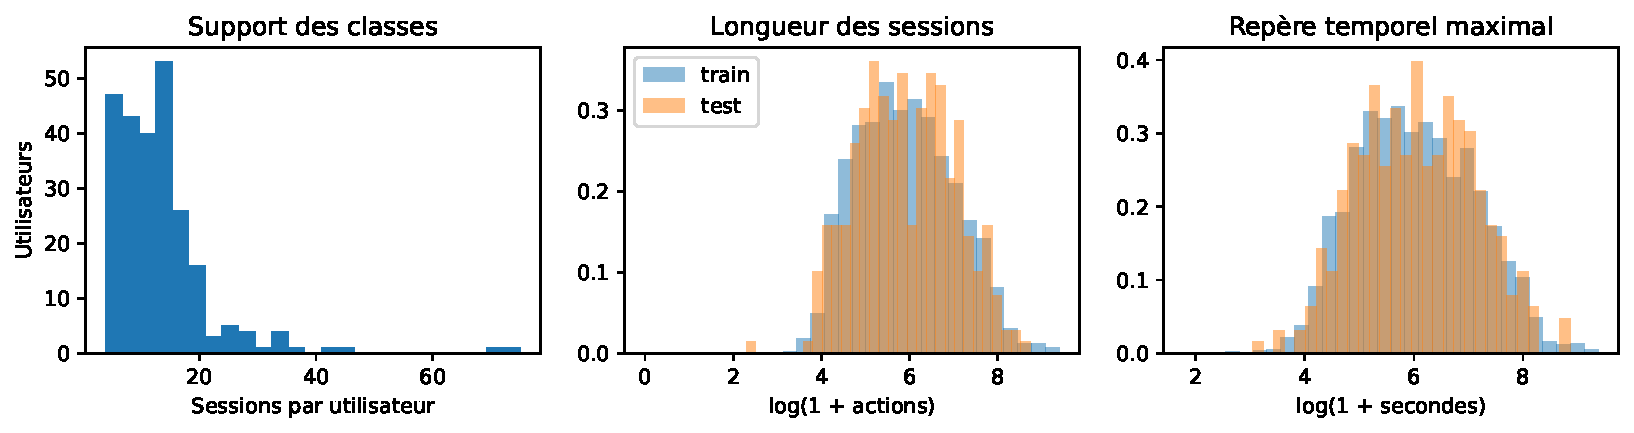
\includegraphics[width=\linewidth]{eda_overview.pdf}
\caption{Vue d'ensemble : distribution des longueurs, entropie d'actions et repères temporels.}
\end{figure}

\section{Construction des caractéristiques}
Toutes les transformations sont ajustées à l'intérieur des plis d'apprentissage. Le tableau
\ref{tab:families} résume les familles; la famille A conserve les événements entiers comme
jetons afin de capturer les séquences d'écrans, la famille C isole le contexte métier, et la
famille E ajoute un profil quantitatif standardisé. Un test verrouille l'absence de fuite: un
jeton ou un navigateur absent des plis d'apprentissage ne peut pas apparaître dans le
vocabulaire, et les transformateurs non ajustés restent inchangés.
\begin{table}[htbp]
\caption{Familles de caractéristiques et hypothèses associées (matrice brute de 45140 colonnes).}
\label{tab:families}
\begin{tabular}{llll}
\toprule
Famille & Contenu & Hypothèse comportementale & Encodage \\
\midrule
A. Actions brutes & Séquence complète des actions/écrans/configs & généalogie du comportement & unigrammes→trigrammes \\
B. Action seule & verbe d'action sans contexte & style d'usage & unigrammes→trigrammes \\
C. Contexte & écran, config, chaîne, paires action-contexte & module métier utilisé & unigrammes→trigrammes \\
D. Position/Temps & début/fin de session, intervalles tNN discrétisés & rythme et point d'entrée & unigrammes positionnels \\
E. Statistiques & statistiques de session (longueur, entropie, resets) & profil quantitatif & 19 variables standardisées \\
\bottomrule
\end{tabular}
\end{table}


\section{Méthodes de classification}
Le protocole réserve d'abord 80\,\% des
sessions de développement; la sélection se fait sur une validation croisée stratifiée à trois
plis de ce sous-ensemble uniquement, avant tout accès au holdout. La comparaison finale
utilise \code{RepeatedStratifiedKFold} (k=4,
3 répétitions) et sert de mesure de stabilité descriptive après
verrouillage du choix. Les métriques sont l'exactitude, la F1-macro, la F1 pondérée,
l'exactitude équilibrée, la précision top-3/top-5 et la log-loss. La règle de choix retient le
modèle pré-déclaré le plus simple à moins d'un écart-type du meilleur; un vote n'est accepté que
s'il gagne de plus d'un écart-type. Les baselines (majoritaire, aléatoire stratifiée,
navigateur seul) figurent dans le tableau \ref{tab:models}.

\section{Résultats}
Le modèle retenu est \code{linear_balanced}. Sur le holdout indépendant, l'exactitude atteint
0.951 et la F1-macro 0.941; en validation croisée
répétée sur le train complet, la F1-macro vaut 0.958 ±
0.009. La calibration sigmoïde interne n'améliore pas la F1-macro de
façon décisive. Les baselines confirment que le signal provient bien des séquences, non du
navigateur ni de la classe majoritaire.
\begin{table}[htbp]
\caption{Comparaison des modèles : moyenne ± écart-type sur 4 plis stratifiés × 3 répétitions (train complet).}
\label{tab:models}
\begin{tabular}{lrrrrrrrr}
\toprule
Modèle & Acc & ± & F1-macro & ± & Acc. équil. & Top-5 & Log-loss & Temps (s) \\
\midrule
majority & 0.023 & 0.001 & 0.000 & 0.000 & 0.004 & 0.039 & 35.219 & 1.004 \\
random & 0.006 & 0.003 & 0.004 & 0.002 & 0.004 & 0.022 & 35.813 & 1.148 \\
browser & 0.051 & 0.001 & 0.005 & 0.000 & 0.016 & 0.176 & 4.313 & 0.006 \\
linear & 0.961 & 0.005 & 0.948 & 0.007 & 0.949 & 0.993 & 4.083 & 4.070 \\
logistic & 0.785 & 0.007 & 0.639 & 0.010 & 0.651 & 0.924 & 2.686 & 17.110 \\
ridge & 0.933 & 0.006 & 0.902 & 0.010 & 0.904 & 0.990 & 4.592 & 8.902 \\
complement\_nb & 0.803 & 0.012 & 0.713 & 0.016 & 0.728 & 0.964 & 4.466 & 1.327 \\
rbf & 0.928 & 0.008 & 0.896 & 0.010 & 0.894 & 0.967 & 1.042 & 15.883 \\
forest & 0.912 & 0.008 & 0.879 & 0.016 & 0.881 & 0.983 & 1.191 & 6.201 \\
extra\_trees & 0.923 & 0.010 & 0.893 & 0.014 & 0.895 & 0.984 & 1.100 & 5.419 \\
hist\_gradient & 0.724 & 0.012 & 0.659 & 0.015 & 0.659 & 0.848 & 1.757 & 4.330 \\
mlp & 0.924 & 0.005 & 0.911 & 0.008 & 0.916 & 0.983 & 0.299 & 4.189 \\
knn & 0.910 & 0.009 & 0.900 & 0.007 & 0.902 & 0.960 & 1.601 & 1.016 \\
soft\_vote & 0.911 & 0.007 & 0.875 & 0.015 & 0.876 & 0.983 & 1.971 & 21.554 \\
stacking & 0.447 & 0.013 & 0.281 & 0.008 & 0.272 & 0.523 & 4.218 & 18.901 \\
sgd\_elasticnet & 0.912 & 0.009 & 0.865 & 0.013 & 0.868 & 0.977 & 1.543 & 7.038 \\
poly & 0.930 & 0.007 & 0.903 & 0.011 & 0.900 & 0.971 & 0.953 & 15.462 \\
linear\_unigrams & 0.927 & 0.003 & 0.899 & 0.009 & 0.904 & 0.989 & 3.982 & 0.705 \\
linear\_balanced & 0.966 & 0.005 & 0.958 & 0.009 & 0.961 & 0.993 & 4.126 & 3.355 \\
\bottomrule
\end{tabular}
\end{table}


\begin{figure}[htbp]\centering
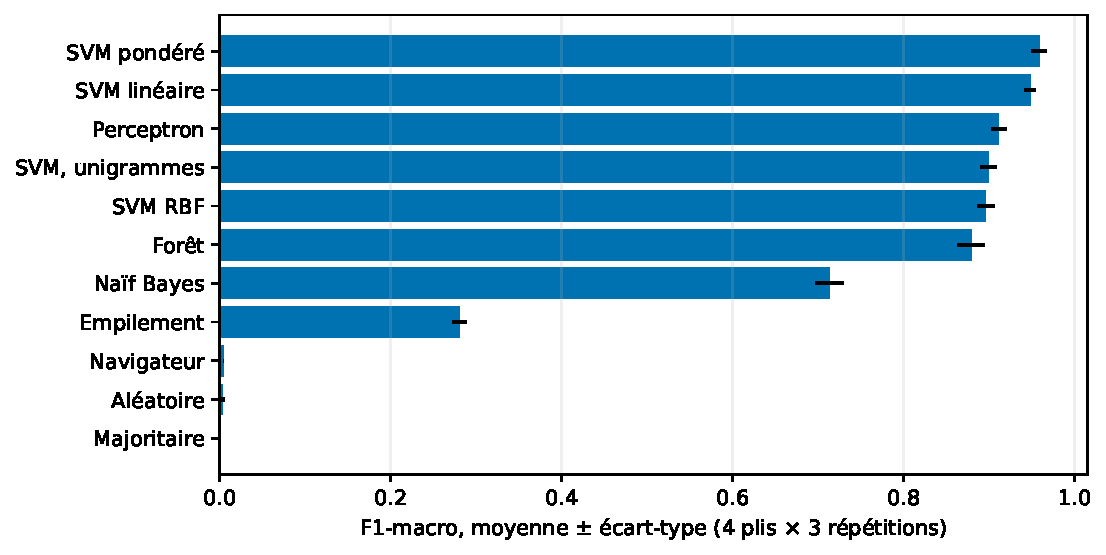
\includegraphics[width=0.9\linewidth]{model_comparison.pdf}
\caption{Comparaison des modèles (moyenne ± écart-type, 4 plis × 3 répétitions).}
\end{figure}

\subsection{Ablations et courbe d'apprentissage}
Les ablations par famille (tableau \ref{tab:permutation}) et la courbe
d'apprentissage (tableau \ref{tab:learning}, figure suivante) sont des diagnostics
post-verrouillage; elles n'ont pas servi à choisir le modèle.
\begin{table}[htbp]
\caption{Permutation groupée par famille sur le holdout (perte de F1-macro).}
\label{tab:permutation}
\begin{tabular}{lrrr}
\toprule
Famille & Colonnes & Perte F1-macro & Écart-type \\
\midrule
raw & 39326 & 0.933 & 0.003 \\
browser & 4 & 0.113 & 0.009 \\
\bottomrule
\end{tabular}
\end{table}

\begin{table}[htbp]
\caption{Courbe d'apprentissage du modèle retenu (diagnostic post-verrouillage).}
\label{tab:learning}
\begin{tabular}{rrrr}
\toprule
fraction & train\_sessions & train\_macro\_f1 & holdout\_macro\_f1 \\
\midrule
0.350 & 853 & 1.000 & 0.890 \\
0.650 & 1583 & 1.000 & 0.908 \\
1.000 & 2623 & 1.000 & 0.941 \\
\bottomrule
\end{tabular}
\end{table}

\begin{figure}[htbp]\centering
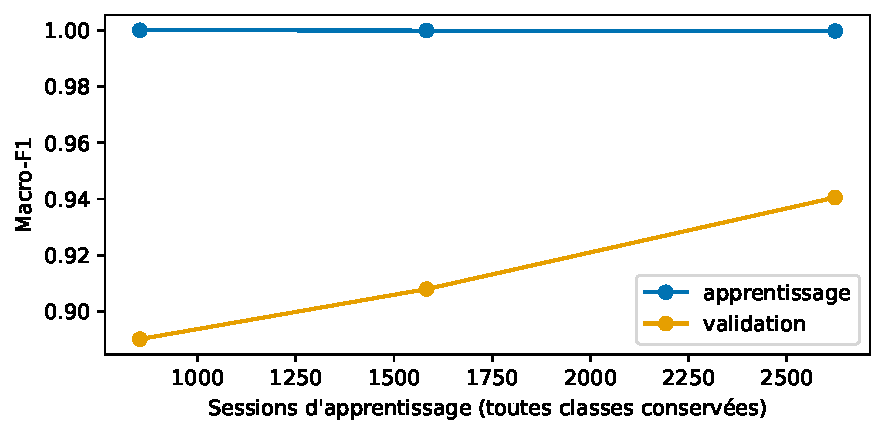
\includegraphics[width=0.6\linewidth]{learning_curve.pdf}
\caption{Courbe d'apprentissage : macro-F1 train et holdout selon la taille d'apprentissage.}
\end{figure}

\subsection{Analyse des erreurs}
L'exactitude baisse sur les sessions très courtes, où le signal disponible est faible, alors que
les sessions longues restent bien classées; le tableau \ref{tab:length} le quantifie. Les
confusions se concentrent entre utilisateurs partageant les mêmes modules (tableau
\ref{tab:confusion}), ce qui suggère des rôles ou habitudes proches.
\begin{figure}[htbp]\centering
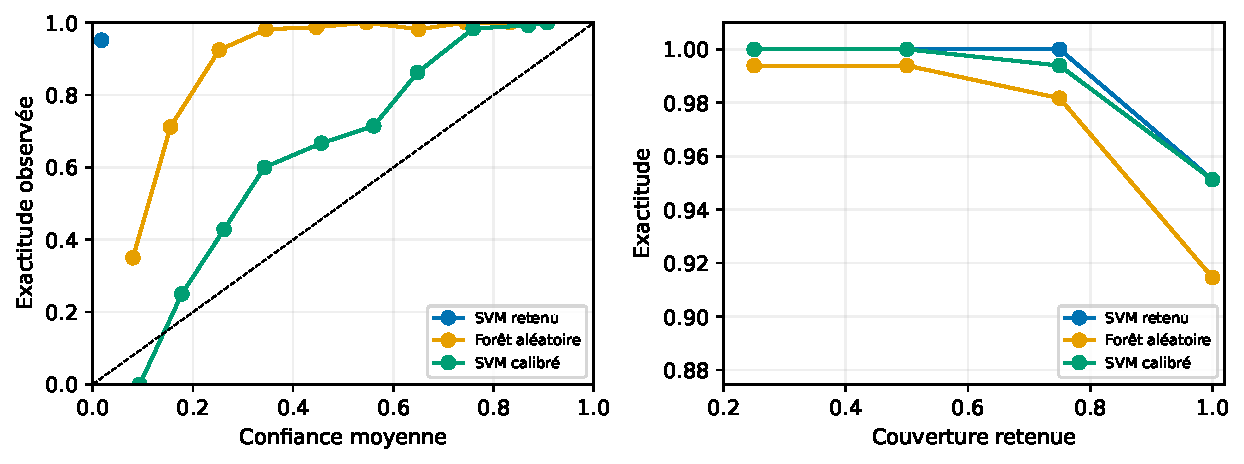
\includegraphics[width=\linewidth]{confidence.pdf}
\caption{Fiabilité (gauche) et exactitude selon la couverture d'abstention (droite).}
\end{figure}
\begin{table}[htbp]
\caption{Exactitude par tranche de longueur de session (holdout).}
\label{tab:length}
\begin{tabular}{lrr}
\toprule
Longueur (tokens) & Exactitude & Sessions \\
\midrule
0-100.0 & 0.902 & 41 \\
100-500.0 & 0.923 & 323 \\
2000+ & 1.000 & 66 \\
500-2000.0 & 0.987 & 226 \\
\bottomrule
\end{tabular}
\end{table}

\begin{table}[htbp]
\caption{Principales confusions sur le holdout.}
\label{tab:confusion}
\begin{tabular}{llr}
\toprule
Vérité & Prédit & Occurrences \\
\midrule
skm & slq & 2 \\
akx & hvh & 1 \\
ajo & szr & 1 \\
azn & wht & 1 \\
azx & guh & 1 \\
bos & czi & 1 \\
ald & fuy & 1 \\
flj & skm & 1 \\
\bottomrule
\end{tabular}
\end{table}


\section{Interprétabilité et discussion}
\textbf{Confiance.} L'ECE mesuré sur le holdout est
0.934. Le SVM natif n'expose pas de
probabilités; la log-loss et la fiabilité reposent sur un softmax de marges explicitement non
calibré, ou sur la calibration sigmoïde interne. L'analyse d'abstention montre qu'une couverture
réduite augmente l'exactitude (figure précédente).
\textbf{Explication locale.} Pour le modèle retenu, la contribution d'un jeton est exactement
\code{coefficient $\times$ valeur TF-IDF} plus l'ordonnée à l'origine; pour la forêt aléatoire,
nous fournissons une décomposition exacte des probabilités le long des chemins, sans prétendre à
des valeurs de Shapley. Un arbre de profondeur 2 sur les statistiques denses illustre des règles
lisibles.
\begin{figure}[htbp]\centering
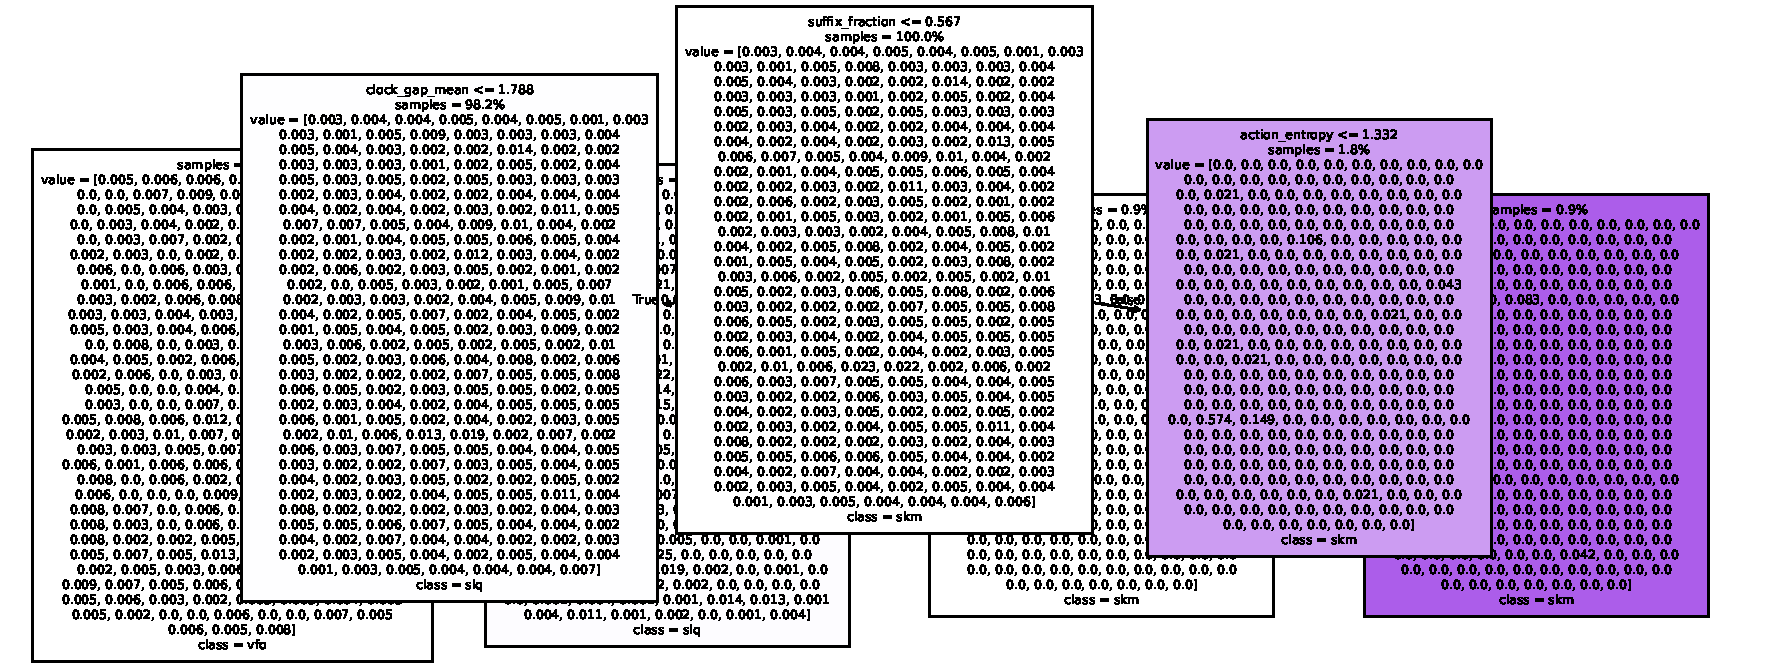
\includegraphics[width=\linewidth]{pruned_tree.pdf}
\caption{Arbre de profondeur 2 sur statistiques denses (illustration pédagogique, pas le modèle retenu).}
\end{figure}
\textbf{Variables influentes et redondance.} La permutation groupée (tableau
\ref{tab:permutation}) montre l'apport des familles A/C; les motifs récurrents
(écran\,$\to$\,action) ont un sens comportemental. La sélection de représentants de clusters
permet de retirer des colonnes redondantes avec une perte mesurée, documentée dans
\code{interpretability.json}.
\textbf{Limites.} 247 classes avec peu de sessions chacune, dérive temporelle,
test de 324 lignes bruité, et ré-identification potentielle des
utilisateurs: autant de raisons de préférer un modèle simple et validé à un score fragile.

\section{Conclusion}
Une chaîne linéaire TF-IDF + SVM, correctement validée hors pli, explique la majorité des
sessions; les modèles plus complexes n'apportent pas de gain supérieur à un écart-type. Les
prochaines étapes incluent l'augmentation par fenêtres pour les classes rares et une analyse
d'équité par utilisateur, sous contrainte de confidentialité. La soumission
\code{submission_20261013T192402Z_linear_balanced.csv} (empreinte
\code{3ff5121962f6}) est régénérée par \code{make predict}.

\end{document}
